\chapter{Violación CP}\label{cap:CP_violation}
Los conceptos de paridad y violación de paridad han sido utilizados varias veces en los capítulos anteriores, pero no hemos explicado en qué consisten en ningún momento. Antes de comenzar con la descripción de los mesones $\PK$ neutros y la violación CP, resulta útil dar unas pinceladas sobre el concepto de paridad y qué papel jugaron los kaones en el descubrimiento de su violación en la fuerza débil. 

Cuando ciertas propiedades de una partícula no cambian al someterla a un conjunto de transformaciones, se dice que esa partícula tiene una simetría. De acuerdo con el Teorema de Noether, cada simetría se asocia a una magnitud física que se conserva, las cuales se describen mediante operadores hermíticos. Hay dos simetrías discretas importantes que conviene discutir en relación con los mesones $\PK$, ya que en la interacción fuerte y en la
electromagnética se conservan, pero pueden violarse en la interacción débil. Estas dos simetrías son la inversión espacial P y la conjugación de carga C.

En la invariancia frente a la inversión espacial o simetría P (a veces, paridad) se invierte el signo de las coordenadas de las partículas. En consecuencia, los pseudoescalares y los vectores polares cambian su signo (ejemplos de vectores polares son la posición $\vec{r}$ y el momento lineal $\vec{p}$), mientras que los escalares y los vectores axiales o pseudovectores lo conservan (ejemplos de vectores axiales son el momento angular orbital $\vec{l}$ o el espín $\vec{s}$). Esta simetría se describe mediante el operador paridad $\hat{P}$. La paridad intrínseca o paridad-P $\eta _{P}\left(A \right)$ se determina empíricamente y se asocia con la estructura interna de la partícula A, pudiendo ser su valores $\pm 1$. Para fermiones y bosones se tiene $\eta _{P}\left(f \right)= -\eta_{P} \left(\overline{f} \right)$ y $\eta_{P}\left(b \right)=\eta_{P}\left(\overline{b}\right)$, respectivamente \cite{notas2020}. 

De forma similar, la invariancia frente a la conjugación de carga o simetría C, transforma partículas A en antipartículas $\overline{A}$ y viceversa, de modo que cambia el signo de la carga y del resto de números cuánticos internos (número bariónico $B$, número leptónico $L$, extrañeza $S$, etc.), dejando intactos la masa, la energía, el momento y el espín.  El operador asociado es $\hat{C}$. Nuevamente, $\eta _{C}\left(A\right)= \pm 1$. En este caso, sólo las partículas neutras tienen la paridad-C  $\eta _{C}\left(A \right)$ bien definida \cite{notas2020}. 

Estas dos simetrías parecen conservarse siempre en los procesos donde intervenían interacciones fundamentales. Sin embargo, el hallazgo de los mesones $\PK$ trajo consigo las primeras evidencias de que la interacción débil podía violar las simetrías P y C.


\subsubsection{Enigma $\Ptau$-$\theta$}
Tras las primeras observaciones de los mesones $\PK$ en los años 50, había un par decaimientos de estas, por entonces llamadas, partículas $V$ que desconcertaba a los científicos de la época. Tanta era la confusión que incluso se llegó a pensar que había dos tipos de partículas $V$, a las que denominaron $\Ptau$ y $\theta$, como se mencionó en el capítulo \ref{cap:strangeness}. 

Recordemos que, por una parte, en la fotografía \ref{fig:nature1}, se observaba el decaimiento $\theta^{0} \rightarrow \Ppiplus\Ppiminus$ y años más tarde también se había constatado la existencia del proceso $\theta^{+} \rightarrow \Ppiplus\Pgpz$. Por otro lado, la fotografía \ref{fig:powell} mostraba la desintegración de $\APtauon \rightarrow \Pgpp\Pgpp\Pgpm$.  El estudio de estos dos procesos concluía que las partículas $\Ptau$ y $\theta$ eran idénticas pues tenían las mismas masas, las mismas vidas medias, etc., pero dado que los decaimientos tenían distinta paridad, era \textit{imposible} que fueran las mismas partículas; no se concebía que la paridad fuera violada. Esto hecho fue conocido como el \textit{enigma $\Ptau$-$\theta$} \cite{Ferbel}.
\begin{equation}
\begin{gathered}
\theta^{+} \rightarrow \pi^{+}\pi^{0} \Rightarrow \eta_{P}\left(\pi^{+}\right) \eta_{P}\left(\pi^{+}\right) = 1 \\ 
\tau^{+} \rightarrow \pi^{+}\pi^{+}\pi^{-} \Rightarrow \eta_{P}\left(\pi^{+}\right) \eta_{P}\left(\pi^{+}\right) \eta_{P}\left(\pi^{-}\right) = -1
\end{gathered}
\end{equation}
En 1956, Lee y Yang estudiaron a fondo el rompecabezas, concluyendo que no había ninguna evidencia para afirmar que la paridad se conservara en la interacción débil, por lo que las partículas $\tau$ y $\theta$ debían ser la misma y la violación de la paridad en esta interacción era una realidad más que plausible. 

El experimento clave que corroboró esta hipótesis, realizado por Wu y Ambler, consistió en analizar la emisión $\beta$ del $\tensor*[^{60}]{\mathrm{Co}}{}$ polarizado (por ser semejante a la del neutrón): 
\begin{equation}
\tensor*[^{60}]{\mathrm{Co}}{} \longrightarrow \tensor*[^{60}]{\mathrm{Ni}}{} + \Pem + \APnu_{e}
\end{equation}
utilizando un campo magnético externo, se polarizan los espines de un cristal de cobalto radioactivo previamente enfriado a $\SI{0,01}{\kelvin}$, minimizando así su despolarización por agitación térmica. Cuando el núcleo de cobalto decae, se miden las direcciones de los electrones emitidos. Wu y Ambler notaron que, preferentemente, los $\Pem$ se emitían en una dirección paralela al campo y, por lo tanto, igual a la dirección de espín del núcleo padre. Esto es, si el campo apuntaba al norte, los $\Pem$ se emitían por el norte. Para que la paridad se conserve, si se repite el mismo experimento alineando el espín nuclear nuevamente, pero ahora en dirección sur, los $\Pem$ deberían salir por el sur esta vez. No obstante, se observó que este no era el caso y los electrones seguían mostrando preferencia por emitirse en dirección norte, constatado así la violación de simetría P en la interacción débil \cite{Ferbel} \cite{Griffiths2008}. 

\begin{figure}[!ht]
\begin{subfigure}[t]{.5\textwidth}
  \centering
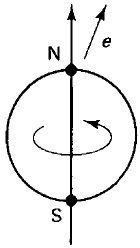
\includegraphics[width=0.4\linewidth]{{C:/Users/Carmen/Desktop/Universidad/TFG/Borradores/img/cobalto1.PNG}}
\caption{$\Pem$ emitido en la dirección del campo.}
  \label{fig:cobalto1}
\end{subfigure}%
\begin{subfigure}[t]{.5\textwidth}
  \centering
  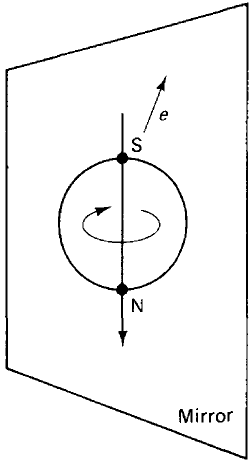
\includegraphics[width=0.45\linewidth]{{C:/Users/Carmen/Desktop/Universidad/TFG/Borradores/img/cobalto2.PNG}}
  \caption{$\Pem$ emitido dirección opuesta al campo.}
  \label{fig:cobalto2}
\end{subfigure}
\caption[Experimento de Wu y Ambler]{Evidencia de la violación P en el experimento de Wu.  \cite{Griffiths2008}}
\label{fig:cobalto}
\end{figure}


Hasta mediados de los 50, los científicos asumían que la mitad de los neutrinos tendrían helicidad positiva y la otra mitad helicidad negativa. La implicación verdaderamente importante que tuvo descubrir la violación P en la fuerza débil fue que sólo existían neutrinos con helicidad negativa y antineutrinos con helicidad positiva. 

Siguiendo la misma línea de razonamiento, si aplicásemos la conjugación de carga a un neutrino (que tiene helicidad negativa), nos daría un antineutrino. Pero como la paridad-C no cambia el espín, el $\APnu$ resultante mantendría la helicidad negativa del $\Pnu$ original. Y ya hemos confirmado mediante el experimento de Wu que esto no es posible, pues sólo existen antineutrinos con helicidad positiva. Por ende, la interacción débil también presenta violación de simetría C.

Entonces, tras descubrir que la fuerza débil no respetaba las simetrías P y C e intentando unificar las propiedades de las fuerzas fundamentales, se formuló que la combinación de ambas simetrías o simetría CP era lo que realmente debía conservarse.

No obstante, en 1964, el estudio de los decaimientos de mesones $\PKz$ evidenció la violación CP en la interacción débil. La siguiente sección presenta una descripción detallada del decaimiento de los mesones $\PKz$, la violación CP y sus implicaciones.

\section{Decaimiento de mesones $\PK$ neutros}
\label{sec:neutral_kaon_decay}

Volvamos a la época entre 1953 y 1955, relatada en el capítulo \ref{cap:strangeness}. El concepto de extrañeza acababa de surgir y la propuesta de Nishijima se basaba en clasificar los mesones $\PK$ en dobletes de carga, uno para las partículas $\PKp$ y $\PKz$ asignándoles un valor de extrañeza $S=1$, y otro para las correspondientes antipartículas $\PKm$ y $\PaKz$, con $S=-1$.

La teoría parecía clara pero, en el laboratorio, ¿cómo es posible distinguir $\PKz(S=1)$ de $\PaKz(S=-1)$? Esta pregunta, planteada por Fermi, obtuvo su respuesta al formularse un nuevo concepto: los \textit{estados mixtos} (o \textit{mezcla}) de las partículas. Para entender esta nueva hipótesis sobre ``mezcla de partículas'', utilizamos el mismo ejemplo que expone Pais en su libro \cite{Pais}:

Si al decaimiento $\PKz \left(\Pqd\Paqs\right) \rightarrow \Pgpp + \Pgpm$, con amplitud A, le aplicamos una conjugación de carga C, el decaimiento resultante es $\PaKz \left(\Pqs\Paqd\right) \rightarrow \Pgpp + \Pgpm$, también de amplitud A. Se observa que el estado final es el mismo para ambos procesos, pero el inicial no, al tener diferente extrañeza. Esto es debido a que la extrañeza no tiene por qué conservarse en la fuerza débil. Entonces, se tiene que $\PKz$ y $\PaKz$ se mezclan como $\PKz \leftrightarrows \Pgpp + \Pgpm \leftrightarrows \PaKz$.

Cabe destacar que todo este desarrollo fue concebido varios años antes al descubrimiento de la violación P y C en la interacción débil, por lo que haciendo uso de las operaciones P, C y CP, se obtienen las combinaciones\protect\footnotemark de estados siguientes:
\begin{align}
|\PK_{1}\rangle &= \dfrac{|\PKz\rangle - |\PaKz\rangle}{\sqrt{2}} & |\PK_{2}\rangle &= \dfrac{|\PKz\rangle + |\PaKz\rangle}{\sqrt{2}}\label{eq:k1k2def}
\end{align}
ya que los estados de los kaones son pseudoescalares y se cumple que \cite{Griffiths2008}
\begin{align}
P|\PKz\rangle &= -|\PKz\rangle & P|\PaKz\rangle &= -|\PaKz\rangle\\
C|\PKz\rangle &= |\PaKz\rangle & C|\PaKz\rangle &= |\PKz\rangle\\
CP|\PKz\rangle &= -|\PaKz\rangle & CP|\PaKz\rangle &= -|\PKz\rangle
\end{align}

\footnotetext{Los kaones se producen por interacción fuerte, siendo autoestados de la extrañeza, pero al decaer por interacción débil, son autoestados de CP, pudiéndose definir estas combinaciones. Los estados $|\PKz\rangle$ y $|\PaKz\rangle$ son estados descritos por su estructura de quarks mientras $|\PK_{1}\rangle$ y $|\PK_{2}\rangle$ son autoestados de CP.}

Esto implicaba que, \textit{asumiendo} que la paridad conjunta CP se conserve en la interacción débil, $\PK_{1}$ sólo puede decaer en estados pares, es decir con CP=+1 mientras que $\PK_{2}$ sólo decae a estados impares con CP=-1, por lo que $\PK_{1}$  puede decaer a $\Pgpp \Pgpm$ en (con amplitud $A/ \sqrt{2}$) pero $\PK_{2}$ no (amplitud nula). En consecuencia, $\PK_{1}$ y $\PK_{2}$ tienen vidas medias diferentes $\tau_{1}$ y $\tau_{2}$, respectivamente \cite{Pais} \cite{Perkins}.

\begin{figure}[!ht]
	\centering
	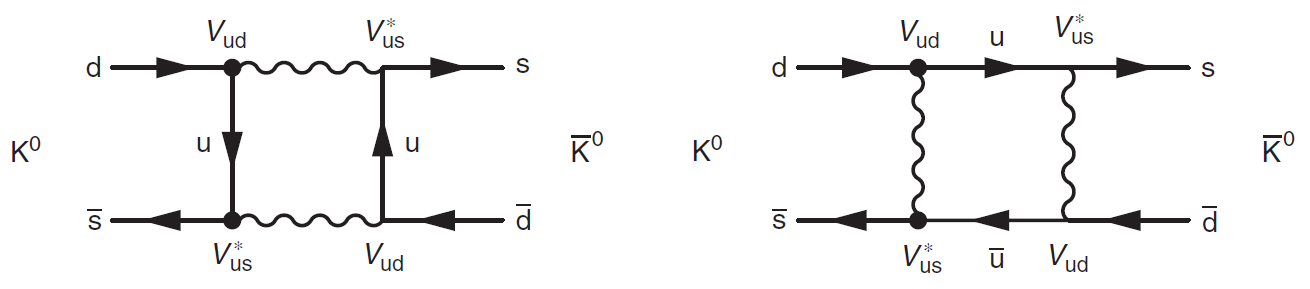
\includegraphics[width=0.9\textwidth]{C:/Users/Carmen/Desktop/Universidad/TFG/Borradores/img/mixing.png}
	\caption[Diagrama de Feynmann de la mezcla de mesones $\PK$ neutros]
	{Diagrama de Feynman de la mezcla de mesones $\PK$ neutros. \cite{Thomson}}
	\label{fig:kaonmix}
\end{figure}

Dado que, típicamente, la designación de partícula se asigna a aquella con una semivida definida, es más correcto expresar la mezcla de estados como \cite{Pais}:
\begin{align}
|\PKz\rangle &= \dfrac{|\PK_{1}\rangle + |\PK_{2}\rangle}{\sqrt{2}} & |\PaKz\rangle &= \dfrac{|\PK_{1}\rangle - |\PK_{2}\rangle}{\sqrt{2}}\label{eq:k1k2defbuena}
\end{align}
Pero ambos sets \ref{eq:k1k2def} y \ref{eq:k1k2defbuena} pueden utilizarse según el que más convenga en cada momento.

Generalmente, los mesones $\PK$ neutros decaen por interacción débil en dos o en tres piones. Al comienzo de este capítulo, comentábamos en el enigma $\Ptau$-$\theta$ que el modo $2\Pgp$ tiene P=+1 y CP=+1 mientras que el de $3\Pgp$ tiene P=-1 y CP=-1 (ambos procesos tienen C=+1). Luego, se concluyó que $\PK_{1}$ decae siempre en $2\Pgp$ mientras $\PK_{2}$ lo hace en $3\Pgp$, asumiendo la invariancia CP. Ahora, dado que la desintegración en $2\Pgp$ es mucho más abundante y más rápida porque libera más energía que el modo $3\Pgp$, tiene una vida media más corta, así $\tau_{2} \gg \tau_{1}$. 

De hecho, esto era lo que los científicos observaban en el laboratorio: únicamente podían distinguir entre un kaón de vida corta $\PKzS$ (short-lived o $\PK$-short) y un kaón de vida larga $\PKzL$ (long-lived o $\PK$-long). Si se conserva la simetría CP, $\PKzS$ y $\PKzL$ se identifican con $\PK_{1}$ y $\PK_{2}$, respectivamente. Además, los estudios empíricos también indicaron que la masa de $\PKzL$ es ligeramente mayor que la de $\PKzS$: 
\begin{equation}
m\left(\PKzL\right)-m\left(\PKzS\right)=\SI{3,5e-6}{\eV}
\end{equation}

Al tener $\PKzL$ más masa, es más pesado y no se mueve tan rápidamente como $\PKzS$, siendo así $\PKzL$ más estable y alcanzando distancias mayores; tiene sentido que $\tau_{2}$ sea mayor que $\tau_{1}$. Por lo tanto, los mesones $\PK$ neutros se propagan como autoestados de masa, pues $\PKzS$ y $\PKzL$ son los estados con masa bien definida.

Experimentalmente, $\tau\left(\PKzL\right) \approx 570\tau\left(\PKzS\right)$ \cite{Zyla}:
\begin{align}
\tau\left(\PKzS\right) &= \SI{8,954(4)e-11}{\second} & \tau\left(\PKzL\right) &= \SI{5,116(21)e-8}{\second}
\end{align}

Sin embargo, al año siguiente, en 1956, se resolvió el enigma $\Ptau$-$\theta$ descubriéndose la violación de paridad P y C en la interacción débil y postulando que la simetría invariante era la CP. El escepticismo acerca de esta hipótesis estaba presente en la comunidad científica. Por este motivo, durante los siguientes años, se estudiaron en profundidad los distintos modos de decaimiento débil de los mesones $\PK$ neutros, analizando la conservación de simetría CP.

En 1964, el grupo de Cronin y Fitch, obtuvo la primera evidencia de violación CP en la interacción débil al observar un decaimiento de $\PKzL$ en dos piones: $\PKzL \rightarrow \Pgpp\Pgpm$.

El experimento que descubrió la violación CP consistía en una fuente que emitía un haz de kaones neutros, el cual seguidamente era colimado y atravesaba un tubo largo. Como se ha comentado anteriormente, $\PKzL$ puede alcanzar una mayor distancia de propagación al tener una semivida mayor que $\PKzS$. Esto implica que al detector situado en el extremo final del tuvo únicamente llegaba un haz de mesones $\PKzL$ puro. La gran mayoría de desintegraciones detectadas eran decaimientos en $3\pi$. Sin embargo, también midieron algunos decaimientos de $\PKzL$ en $2\pi$. Los modos $\PKzL \rightarrow 2\Pgp$ eran muchísimo menos numerosos, de un total de 22700 decaimientos detectados sólo $45 \pm 9$ correspondían al modo $2\Pgp$ \cite{Cronin}. Además, estos procesos se caracterizaban porque el valor de CP a ambos lados de los mismos no coincidía, ergo se violaba la simetría CP:
\begin{align}
CP\left(\PKzL\right) &=-1 & CP\left(\Pgpp\Pgpm\right) &= +1
\end{align}

Básicamente, se formularon dos posibles explicaciones para este descubrimiento.
La primera de ellas consiste en mantener la correspondencia entre los autoestados CP y los autosestados de masa $\PKzS \leftrightarrow \PK_{1}$ y $\PKzL \leftrightarrow \PK_{2}$, simplemente asumiendo que hay una \textit{violación CP directa}.

La segunda hipótesis (la más aceptada) aboga por una \textit{violación CP indirecta}. Para ello, redefine los estados de propagación $\PKzS$ y $\PKzL$ como una combinación de los autoestados $\PK_{1}$ y $\PK_{2}$, para incluir una pequeña parte $\epsilon$ del otro autoestado CP (ver eq. \ref{eq:kLkSmix}). Así, $\PKzS$ y $\PKzL$ no son autoestados puros de CP como en un principio se pensaba \cite{Helsinki}.

\begin{align}
|\PKzS\rangle &= \dfrac{1}{\sqrt{1+\left| \epsilon\right| ^{2}}}\left( \left| \PK_{1}\rangle +\epsilon \right| \PK_{2}\rangle \right) &
|\PKzL\rangle &= \dfrac{1}{\sqrt{1+\left| \epsilon\right| ^{2}}}\left( \left| \PK_{2}\rangle +\epsilon \right| \PK_{1}\rangle \right)\label{eq:kLkSmix}
\end{align}
donde $\epsilon$ es un parámetro complejo que mide la desviación de la invariancia CP y cuyo valor se determina empíricamente: $\num{1,596(13)e-3}$ \cite{Zyla}.

Además de en los kaones neutros, la violación CP no se volvió a observar en otras partículas hasta el descubrimiento de los mesones $\PB$ y $\PD$. Su efecto es tan pequeño que aún no se ha encontrado una manera ``natural'' de incluirlo en el formalismo débil, pero hay varias teorías. En el Modelo Estándar, una de ellas se basa en definir la fase $\delta$ de la matriz CKM como compleja para incluir los efectos producidos por la violación CP. Pese a ello, aún no hay una forma unívoca de determinar este factor ni el resto de elementos de la matriz CKM \cite{Griffiths2008}.

Los decaimientos más comunes de $\PKzS$ y $\PKzL$ se muestran en las siguientes tablas:

\begin{table}[!htb]
\begin{minipage}{.5\linewidth}
    \centering
\begin{tabular}{ c c } 
\toprule
\makecell{Mesón $\PKzS$}  &  $BR$ \\
\midrule   
$\Pgpp\Pgpm$ & $69.2\%$ \\
$\Pgpz\Pgpz$ & $30.7\%$ \\
$\Pgpz\Pgpz\Pgpz$ & $<\num{2.6e-8}$ \\
$\Pgpp\Pgpm\Pgpz$ & $\num{3.5e-7}$ \\ \hdashline
$\Pgpm\Pepm\Pnue$ & $0,07\%$ \\
\bottomrule
\end{tabular}
\caption[Modos de decaimiento de $\PKzS$]{Modos y $BR$ de $\PKzS$. \cite{Helsinki}\cite{Zyla}}
\label{tab:KpzS_decay}
\end{minipage}\hfill
\begin{minipage}{.5\linewidth}
    \centering
\begin{tabular}{ c c } 
    \toprule
    \makecell{Mesón $\PKzL$}  &  $BR$ \\    
    \midrule
$\Pgpp\Pgpm$ & $0.20\%$ \\
$\Pgpz\Pgpz$ & $0.09\%$ \\
$\Pgpz\Pgpz\Pgpz$ & $19.5\%$ \\
$\Pgpp\Pgpm\Pgpz$ & $12.5\%$ \\ \hdashline
$\Pgpm\Pepm\Pnue$ & $40,55\%$ \\
    \bottomrule
\end{tabular}
\caption[Modos de decaimiento de $\PKzL$]{Modos y $BR$ de $\PKzL$. \cite{Helsinki}\cite{Zyla}}
\label{tab:KpzL_decay}
\end{minipage}
\end{table}

Otro gran ejemplo donde se aprecia la violación CP es en los decaimientos semileptónicos de $\PKzL$. En la tabla \ref{tab:KpzL_decay} se observa que alrededor de un $33\%$ de los mesones $\PKzL$ decaen en tres piones pero otro $40\%$ lo hacen, o bien en $\Pgpm\Pep\Pnue$ o en $\Pgpp\Pem\APnue$. Nótese que si al primer proceso se le aplica una operación CP se obtiene el segundo proceso. Si la simetría CP fuera invariante, ambos modos semileptónicos serían equiprobables. Sin embargo, los hallazgos experimentales muestran que esto no es del todo así, pues $\PKzL$ muestra una leve preferencia por decaer en el $\Pep$ sobre el $\Pem$, permitiendo discernir entre materia y antimateria claramente. Este hecho sugiere que la violación CP puede ser responsable de que predomine la materia sobre la antimateria en el universo \cite{Griffiths2008}.

\subsection{Oscilaciones de mesones K}\label{sec:kaon_oscillations}



\subsubsection{Teoría Electrodébil}\label{sec:electroweak}
Describir unificación de la interacción débil y la electromagnética
e introducir formalismo $Z^0$